\chapter{Death, Life, And Love}

This chapter follows J. Krishnamurti's dialogue with Dr. Alan W. Anderson on death, life, love, consciousness, reincarnation, and immortality. There are no validated blackboard frames for this lecture, so every diagram and equation below is an editorial reconstruction from the spoken inquiry. The notation is deliberately light: it is used to keep distinctions precise, not to turn the dialogue into a formal psychological system.

\section{The Fear Around Death}

Anderson opens by taking up the thread from the previous conversation. They had been speaking of consciousness, death, living as a total movement, and the word reincarnation. Krishnamurti accepts the continuation, but he does not begin with reincarnation. He begins with the fear around death.

Death is not ordinarily discussed as part of daily life. It is avoided, postponed, softened, and hidden. Krishnamurti even notes the absurdity of making a corpse appear as though death has not taken place. This is not merely a social observation. If the mind is frightened of death, then any inquiry into death is already bent toward comfort, belief, or escape.

The first condition of the inquiry is therefore

\begin{equation}
\text{understanding death}
\quad\Longrightarrow\quad
\text{freedom from fear}.
\end{equation}

The arrow should be read as a condition of inquiry, not as a doctrine. Krishnamurti's striking phrase is that death has beauty, strength, and vitality. We usually treat death as the negation of life; the lecture begins by asking whether that assumption is already the product of fear.

\section{Belief, Preparation, And The Question Of Fact}

Krishnamurti next clears away the inherited answers. The Egyptians prepared for death by taking into the tomb the goods of life. Reincarnation, as commonly believed, imagines continuation in another birth. Resurrection imagines survival beyond the grave. These are different religious and cultural forms, but in this dialogue they have the same structural tendency: they preserve continuity.

\begin{align}
\text{Egyptian preparation} &\Rightarrow \text{carry the known forward}, \\
\text{reincarnation as belief} &\Rightarrow \text{continue the known later}, \\
\text{resurrection as belief} &\Rightarrow \text{preserve the known beyond death}.
\end{align}

The transition is sharp: ``what is the fact?'' The question is not what one believes about death, but what actually dies, apart from the organism. The organism may continue for many years, but a longer life of quarrel, bitterness, jealousy, futility, and fear is still a life of the same content.

Anderson names the link: this whole movement is the content of consciousness. At once the question becomes more exact. We are not frightened of death as an abstraction; we are frightened of losing the known.

\begin{equation}
\text{fear of death}
\sim
\text{fear of losing the known}.
\end{equation}

The known includes house, wife, husband, children, property, bank account, reputation, beliefs, memories, acquired knowledge, and the image of oneself. The inquiry into death is now an inquiry into the structure of consciousness.

\section{The Content Of Consciousness As The Known}

We introduce one piece of notation. Let \(C\) denote the content of consciousness. It includes the conscious and the hidden, the personal and the collective: attachment, dependency, acquisition, power, position, anxiety, fear, pleasure, memory, knowledge, inherited influence, and the residues of living in a disordered world.

The lecture's central identification can be written as

\begin{equation}
C \equiv \text{the known} \equiv \text{the me}.
\end{equation}

This is not a blackboard formula; it is a compact way of preserving the spoken insight. The ``me'' is not a separate observer standing outside the content. The me is the content. Consciousness, in the sense being discussed here, has made its own frontier through what it contains.

Krishnamurti then changes the sense of death. Death is not only the biological ending of the organism. There is a psychological death in which the content that sustains the me comes to an end.

\begin{equation}
\text{emptying } C
\Rightarrow
\text{ending the limitation made by } C.
\end{equation}

But this must not be confused with violent detachment. Krishnamurti uses attachment as an example. I am attached to property, to a person, to a book I have written, to knowledge I have acquired. Seeing that attachment breeds pain, I say, ``I must be detached.'' Then the battle to become detached begins, and that battle itself becomes part of consciousness.

\subsection{Question \& Answer}

\paragraph{Question.}
Can the content of consciousness be totally emptied?

\paragraph{Answer.}
Only if the movement of the content is seen without adding another movement of conflict. Emptying does not mean suppression, forced detachment, or cultivating an opposite state. If attachment gives pain, and the will to become detached gives conflict, then the conflict also belongs to \(C\).

\begin{align}
\text{attachment} &\Rightarrow \text{pain}, \\
\text{will to detach} &\Rightarrow \text{conflict}, \\
\text{conflict} &\subset C.
\end{align}

So the question becomes more demanding: can the whole content be observed, including its unconscious and inherited layers, without creating another struggle inside the same field?

\section{Why Analysis Cannot Empty The Mind}

At this point the modern answer appears naturally: analysis. If consciousness contains hidden, personal, collective, racial, acquired, and transitory material, perhaps analysis can uncover it. Krishnamurti rejects this answer. His phrase is ``analysis, paralysis,'' but the rejection is not a slogan; it has a precise structure.

\begin{proposition}
Analysis cannot empty the content of consciousness because it divides the field, takes time, and carries incompletion forward as memory.
\end{proposition}

\begin{proof}
The argument runs as follows.

\begin{enumerate}
\item Analysis begins with an analyser and the analysed.
\item The analyser is not outside consciousness. The analyser is itself a fragment of the content.
\item Therefore the analyser is the analysed:
\begin{equation}
\text{analyser} = \text{analysed}.
\end{equation}
\item Analysis also requires time. It proceeds by uncovering, interpreting, and continuing.
\item Each analysis is incomplete, or is at least uncertain of completion.
\item That incompletion is carried forward as memory.
\item Memory then becomes the basis from which the next incident is analyzed.
\item Thus analysis repeats the continuity it is supposed to end.
\end{enumerate}

In compact form,

\begin{equation}
\text{analysis}
\Rightarrow
\text{division}
\Rightarrow
\text{time}
\Rightarrow
\text{incompletion}
\Rightarrow
\text{memory}
\Rightarrow
\text{further analysis}.
\end{equation}

The result is paralysis because the method remains inside the field it seeks to empty.
\end{proof}

This is the lecture's most explicit worked structure. Analysis promises revelation, but its mechanism is already the mechanism of continuity. If the mind sees this, analysis falls away. Then the dialogue reaches its real difficulty.

\subsection{Question \& Answer}

\paragraph{Question.}
If analysis falls away, what is the mind to do with the content?

\paragraph{Answer.}
It has to be emptied; otherwise there is mere continuity. But it cannot be emptied by an analyser, because the analyser is the analysed. Therefore the problem is not how to analyze the content piece by piece, but how the whole content can be seen at once, without fragmentation.

\begin{figure}
\centering
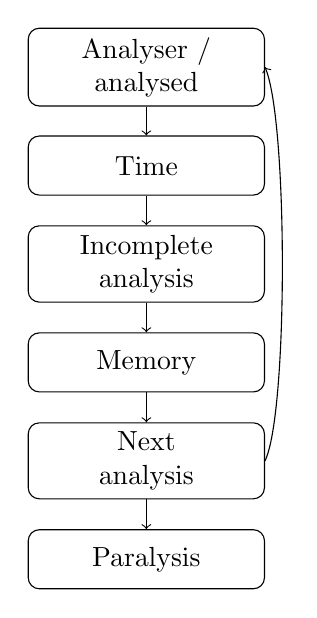
\begin{tikzpicture}[scale=1.0]
\node[draw, rounded corners, align=center, minimum width=3.0cm, minimum height=0.75cm] (a) at (0,0) {Analyser /\\ analysed};
\node[draw, rounded corners, align=center, minimum width=3.0cm, minimum height=0.75cm] (t) at (0,-1.25) {Time};
\node[draw, rounded corners, align=center, minimum width=3.0cm, minimum height=0.75cm] (i) at (0,-2.5) {Incomplete\\ analysis};
\node[draw, rounded corners, align=center, minimum width=3.0cm, minimum height=0.75cm] (m) at (0,-3.75) {Memory};
\node[draw, rounded corners, align=center, minimum width=3.0cm, minimum height=0.75cm] (n) at (0,-5.0) {Next\\ analysis};
\node[draw, rounded corners, align=center, minimum width=3.0cm, minimum height=0.75cm] (p) at (0,-6.25) {Paralysis};

\draw[->] (a) -- (t);
\draw[->] (t) -- (i);
\draw[->] (i) -- (m);
\draw[->] (m) -- (n);
\draw[->] (n) -- (p);
\draw[->] (n.east) .. controls (1.8,-4.4) and (1.8,-0.7) .. (a.east);
\end{tikzpicture}
\caption{Analysis as a loop of division, time, incompletion, memory, and renewed analysis.}
\end{figure}

Anderson then offers a helpful image: we usually think of death laterally, as a terminus on a line. Krishnamurti accepts the point because it fits the analysis just given. The lateral line is the line of repetition. What is being asked is not another endpoint on that line, but a qualitative change.

\begin{figure}
\centering
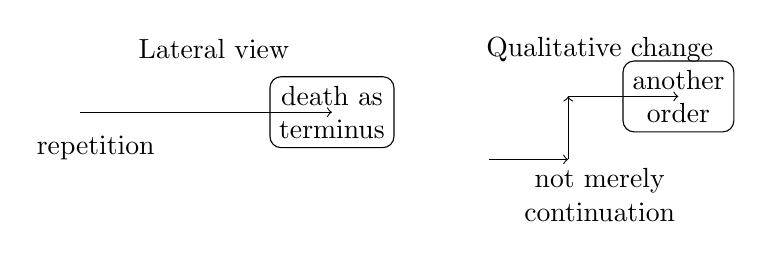
\begin{tikzpicture}[scale=1.0]
\node[align=center] at (-2.5,1.6) {Lateral view};
\draw[->] (-4.2,0.8) -- (-1.0,0.8);
\node[align=center] at (-4.0,0.35) {repetition};
\node[draw, rounded corners, align=center] at (-1.0,0.8) {death as\\ terminus};

\node[align=center] at (2.4,1.6) {Qualitative change};
\draw[->] (1.0,0.2) -- (2.0,0.2);
\draw[->] (2.0,0.2) -- (2.0,1.0);
\draw[->] (2.0,1.0) -- (3.4,1.0);
\node[align=center] at (2.4,-0.25) {not merely\\ continuation};
\node[draw, rounded corners, align=center] at (3.4,1.0) {another\\ order};
\end{tikzpicture}
\caption{Anderson's clarifying metaphor: death as a terminus on a line versus death as qualitative change.}
\end{figure}

\section{The Whole Map Without Direction}

The alternative to analysis is not another technique. Krishnamurti gives the image of a map. If we want to go in a certain direction, we use the map to find a route. Then we do not see the whole map; we see only the part that serves our intention. But if there is no direction, we simply look.

Let \(W\) denote the whole field or map of consciousness. Let \(D\) denote directed search, and let \(A_c\) denote choiceless awareness. Then the contrast is

\begin{align}
D(W) &\Rightarrow \text{a selected route through the map}, \\
A_c(W) &\Rightarrow \text{the whole map exposed}.
\end{align}

This notation is only scaffolding. The point is that direction is already choice. Choice selects, excludes, measures, and pursues. Choiceless awareness is not effortful analysis; it is the seeing of the whole content without a chosen path.

Krishnamurti says that such seeing gives energy to go beyond the content:

\begin{equation}
A_c(C)
\Rightarrow
\text{energy to go beyond } C.
\end{equation}

This is where the lecture turns. We began with fear of death, passed through belief, identified the known as content, saw analysis fail, and now have the possibility of seeing the whole content without direction.

\begin{figure}
\centering
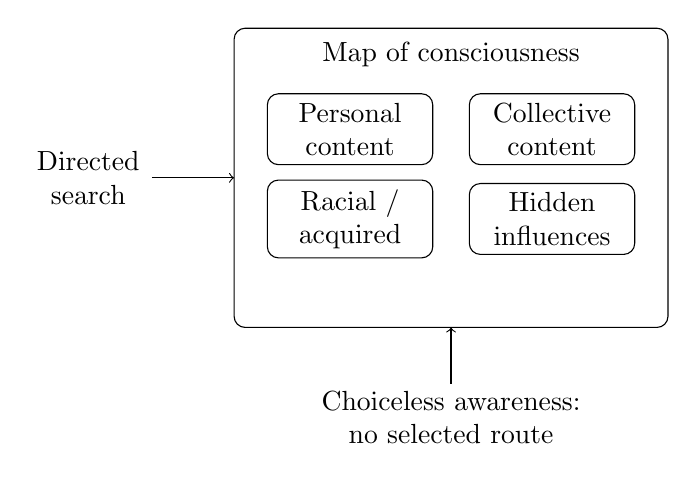
\begin{tikzpicture}[scale=0.95]
\draw[rounded corners] (-2.9,0.0) rectangle (2.9,4.0);
\node[align=center] at (0,3.65) {Map of consciousness};

\node[draw, rounded corners, align=center, minimum width=2.1cm] at (-1.35,2.65) {Personal\\ content};
\node[draw, rounded corners, align=center, minimum width=2.1cm] at (1.35,2.65) {Collective\\ content};
\node[draw, rounded corners, align=center, minimum width=2.1cm] at (-1.35,1.45) {Racial /\\ acquired};
\node[draw, rounded corners, align=center, minimum width=2.1cm] at (1.35,1.45) {Hidden\\ influences};

\draw[->] (-4.0,2.0) -- (-2.9,2.0);
\node[align=center] at (-4.85,2.0) {Directed\\ search};

\draw[->] (0,-0.75) -- (0,0.0);
\node[align=center] at (0,-1.2) {Choiceless awareness:\\ no selected route};
\end{tikzpicture}
\caption{The whole map is not exposed by choosing a direction; it is exposed by looking without choice.}
\end{figure}

\section{Reincarnation Now, Or Continuity As A Stream}

The conversation now returns to reincarnation, but not in its earlier form. At the beginning, reincarnation was one belief among others. Now it is revisited after the analysis of content and continuity.

Krishnamurti's reversal is direct: people speak of reincarnating in a next life, but not of incarnating now. To incarnate now is to die to the content now. Rebirth is not postponed into time; it is linked to the ending of the content that carries time psychologically.

\begin{equation}
\text{incarnation now}
\Longleftrightarrow
\text{dying to } C \text{ now}.
\end{equation}

If the content is not emptied, it continues. Krishnamurti describes it as a river. The content of me is not fundamentally different from the content of you. It is modified by conditioning, exaggerated in different ways, but essentially it is the same human consciousness.

\begin{equation}
C_{\text{unemptied}}
\Rightarrow
\text{continuity like a stream}.
\end{equation}

This stream is not to be turned into a speculative doctrine. In the lecture it names continuity: struggle, pain, unhappiness, fear, accumulation. Krishnamurti says that what appears in mediumistic or seance claims belongs to this continuing stream of content. But a person who has observed and emptied consciousness does not belong to that stream.

\begin{equation}
C_{\text{emptied}}
\Rightarrow
\text{not belonging to the stream}.
\end{equation}

Then one is living each moment anew because one is dying each moment. There is no accumulation of the me which has to be expressed.

\begin{figure}
\centering
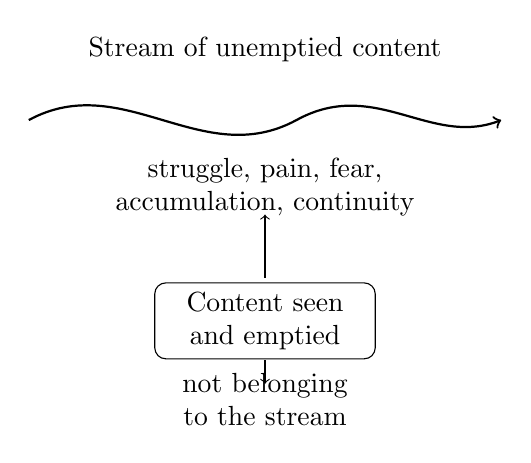
\begin{tikzpicture}[scale=1.0]
\draw[thick, ->] (-3.0,0) .. controls (-1.8,0.65) and (-0.8,-0.65) .. (0.4,0)
                     .. controls (1.4,0.55) and (2.1,-0.35) .. (3.0,0);
\node[align=center] at (0,0.9) {Stream of unemptied content};
\node[align=center] at (0,-0.85) {struggle, pain, fear,\\ accumulation, continuity};

\node[draw, rounded corners, align=center, minimum width=2.8cm] at (0,-2.55) {Content seen\\ and emptied};
\draw[->] (0,-2.0) -- (0,-1.2);

\node[align=center] at (0,-3.55) {not belonging\\ to the stream};
\draw[->] (0,-3.05) -- (0,-3.35);
\end{tikzpicture}
\caption{Unemptied content continues as a stream; emptied content is not another continuation within that stream.}
\end{figure}

\section{Immortality, Beauty, And The Field Of Time}

The dialogue then asks a second great question: what is immortality? Krishnamurti approaches it by negation. It is not the book, the painting, the cathedral, the statue, the family name, the righteous life, the religious ideal, or the god made by thought. All those things can be destroyed or corrupted. More deeply, all are products of thought.

The compact relation is

\begin{equation}
\text{time} = \text{thought}.
\end{equation}

This is not a statement about physical time. It is a claim about psychological continuity: thought creates images, objects, beliefs, ideals, names, and futures. What thought creates belongs to the field of time.

\begin{align}
\text{what thought creates} &\subset \text{the field of time}, \\
\text{thought-made immortality} &\subset \text{the field of time}.
\end{align}

What belongs to time is corruptible. It may last a long while, but it remains destructible. That is why the lecture patiently repeats the negations. Immortality is not in the object, however noble the object may be.

\subsection{Question \& Answer}

\paragraph{Question.}
If immortality is not in works, buildings, beliefs, names, or gods made by thought, what is it?

\paragraph{Answer.}
Krishnamurti distinguishes the object of beauty from beauty itself. A cathedral, poem, sculpture, or painting may perish. The beautiful object can be destroyed. But beauty itself is not the object. It is not grasped as content by consciousness.

\begin{equation}
\text{beautiful object} \in \text{field of time},
\qquad
\text{beauty itself} \notin \text{field of consciousness}.
\end{equation}

Anderson sees the reversal. We usually think beauty dies when the thing we cherished dies. The dialogue turns this around: perhaps beauty has let that expression go. The object perishes; beauty is not imprisoned in it.

\begin{table}
\centering
\begin{tabular}{|p{0.42\linewidth}|p{0.42\linewidth}|}
\hline
Within the field of time & Not treated as within time \\
\hline
Books, paintings, statues, cathedrals & Beauty itself \\
\hline
Family name, reputation, works & The ending of the me \\
\hline
Gods and ideals made by thought & A state not made by thought \\
\hline
Accumulated content and continuity & Living without psychological accumulation \\
\hline
\end{tabular}
\caption{A compact reconstruction of the lecture's contrast between thought-made immortality and what is not contained by thought.}
\end{table}

\section{Living, Love, Death, And Education}

The final movement gathers the chapter into one relation. Death is not merely a future event. The present, in this inquiry, is the death of the content. That is why Anderson's reference to a horizontal track matters: the mind grasps the past or reaches toward the future and never leaves the movement of time.

Krishnamurti's synthesis is severe and simple:

\begin{align}
\text{living} &= \text{dying}, \\
\text{dying to time} &= \text{love}, \\
\text{living},\ \text{love},\ \text{death}
&\Rightarrow
\text{one indivisible movement}.
\end{align}

The transcript appears to misrender one phrase as ``dying to the mean.'' In context the sense is ``dying to the me.'' Love is not what thought calls love: not possession, not pleasure, not merely sex, not the image of another. Love is linked with dying to time and therefore with the ending of the content that divides.

The lecture then turns to education. This is not an appendix. It is the consequence of the whole inquiry. If children are educated only in the cultivation of thought, knowledge becomes the field of psychological safety. Then to die to knowledge, image, and accumulation feels like terror. The self says: this is part of me; how can I let it end?

The movement of wrong education may be summarized as

\begin{equation}
\text{thought as security}
\Rightarrow
\text{fear of not knowing}
\Rightarrow
\text{clinging to } C
\Rightarrow
\text{continuity of the me}.
\end{equation}

Against that stands the movement of perception:

\begin{equation}
\text{actual perception of what is}
\Rightarrow
\text{ending of dissipation}
\Rightarrow
\text{energy in action}
\Rightarrow
\text{transformation not in time}.
\end{equation}

The late transcript is garbled in places, but the surrounding claim is clear: transformation is not produced by an outside agency and is not within the field of time and knowledge. It is the same energy no longer dissipated.

\section{Summary}

The dialogue begins with death and ends with education, but its spine is the movement of consciousness as content. Fear of death is fear of losing the known. The known is the content of consciousness, and that content is the me. Analysis cannot empty the content because the analyser is the analysed, and analysis works through time, incompletion, memory, and repetition.

The alternative is not a new method. It is the seeing of the whole map without direction or choice. From there, reincarnation is transformed into incarnation now: if content is not emptied it continues like a stream; if it is emptied there is no belonging to that stream. Immortality is separated from thought-made objects and linked to beauty itself, not the object of beauty. The chapter closes with the indivisible movement Krishnamurti has been unfolding from the beginning: living, love, and death are not separate fragments in time, but one movement when the content of the me comes to an end.